%%%%%%%%%%%%%%%%%%%%%%%%%%%%%%%%%%%%%%%%%
% Beamer Presentation
% LaTeX Template
% Version 1.0 (10/11/12)
%
% This template has been downloaded from:
% http://www.LaTeXTemplates.com
%
% License:
% CC BY-NC-SA 3.0 (http://creativecommons.org/licenses/by-nc-sa/3.0/)
%
%%%%%%%%%%%%%%%%%%%%%%%%%%%%%%%%%%%%%%%%%

%----------------------------------------------------------------------------------------
%	PACKAGES AND THEMES
%----------------------------------------------------------------------------------------

\documentclass{beamer}
\mode<presentation> {

% The Beamer class comes with a number of default slide themes
% which change the colors and layouts of slides. Below this is a list
% of all the themes, uncomment each in turn to see what they look like.
%\usefonttheme{serif} % default family is serif
%\usefonttheme[onlymath]{serif}

%\usetheme{default}
%\usetheme{AnnArbor}
%\usetheme{Antibes}
%\usetheme{Bergen}
%\usetheme{Berkeley}
%\usetheme{Berlin}
%\usetheme{Boadilla} %Good choice
%\usetheme{CambridgeUS} %Good choice
%\usetheme{Copenhagen}
%\usetheme{Darmstadt}
%\usetheme{Dresden}
%\usetheme{Frankfurt}
%\usetheme{Goettingen}
%\usetheme{Hannover}
%\usetheme{Ilmenau}
%\usetheme{JuanLesPins}
%\usetheme{Luebeck}
\usetheme{Madrid} %Good choice
%\usetheme{Malmoe}
%\usetheme{Marburg}
%\usetheme{Montpellier}
%\usetheme{PaloAlto}
%\usetheme{Pittsburgh}
%\usetheme{Rochester}
%\usetheme{Singapore}
%\usetheme{Szeged}
%\usetheme{Warsaw} %Good choice

% As well as themes, the Beamer class has a number of color themes
% for any slide theme. Uncomment each of these in turn to see how it
% changes the colors of your current slide theme.

%\usecolortheme{albatross}
%\usecolortheme{beaver}
%\usecolortheme{beetle}
%\usecolortheme{crane} 
%\usecolortheme{dolphin}
%\usecolortheme{dove}
%\usecolortheme{fly}
%\usecolortheme{lily}
%\usecolortheme{orchid}
%\usecolortheme{rose}
%\usecolortheme{seagull}
%\usecolortheme{seahorse} %Good choice
%\usecolortheme{whale}
%\usecolortheme{wolverine} %Good choice

%This part is not really crucial
%\useinnertheme{inmargin} %circles, rectanges, rounded, inmargin
%\useoutertheme{tree} %infolines, smoothbars, sidebar, split, tree

%\setbeamertemplate{footline} % To remove the footer line in all slides uncomment this line
%\setbeamertemplate{footline}[page number] % To replace the footer line in all slides with a simple slide count uncomment this line

\setbeamertemplate{navigation symbols}{} % To remove the navigation symbols from the bottom of all slides uncomment this line

%\setbeamertemplate{background canvas}[vertical shading][bottom=white,top=structure.fg!25]
}

\usepackage{tikz}

\usepackage{graphicx} % Allows including images
\usepackage{booktabs} % Allows the use of \toprule, \midrule and \bottomrule in tables
\setbeamercovered{transparent} %This will make the preceding point transparent 
\usefonttheme[onlymath]{serif}
\setbeamertemplate{caption}[numbered]
%\setbeamerfont{title}{family={\fontfamily{Times}}}

%----------------------------------------------------------------------------------------
%	TITLE PAGE
%----------------------------------------------------------------------------------------
\title[This is for short title]{Enter your title here} % The short title appears at the bottom of every slide, the full title is only on the title page

\author{T.O. Ting} % Your name
\institute[XJTLU] % Your institution as it will appear on the bottom of every slide, may be shorthand to save space
{ 
Xian Jiaotong-Liverpool University \\ % Your institution for the title page
\medskip
\textit{toting@xjtlu.edu.cn} % Your email address
}
\date{\today} % Date, can be changed to a custom date

\begin{document}

\begin{frame}
\titlepage % Print the title page as the first slide
\end{frame}

\begin{frame}
\frametitle{Overview} % Table of contents slide, comment this block out to remove it
\tableofcontents % Throughout your presentation, if you choose to use \section{} and \subsection{} commands, these will automatically be printed on this slide as an overview of your presentation
\end{frame}


%----------------------------------------------------------------------------------------
%	PRESENTATION SLIDES
%----------------------------------------------------------------------------------------

%------------------------------------------------
%\section{Structure and Flow} % Sections can be created in order to organize your presentation into discrete blocks, all sections and subsections are automatically printed in the table of contents as an overview of the talk
%------------------------------------------------

%\subsection{Subsection Example} % A subsection can be created just before a set of slides with a common theme to further break down your presentation into chunks

%This part is to display Table of Contents before new section. 
\AtBeginSection[]
{
\begin{frame}{Table of Contents} 
\tableofcontents[currentsection]
\end{frame}
}

%------------------------------------------------
\section{Structure and Flow}
%------------------------------------------------



\begin{frame}{Basic Information }
	\begin{itemize}
		\item<4-> This first point 
		\item<3-> This is third point  
		\item<2->  This is the second point 
	\end{itemize}
\end{frame}


\begin{frame}{Paragraphs of Text}

This is the first paragraph.  This paragraph can be a few lines, ideally not more than six lines in a paragraph.  A long paragraph for presentation tends to be boring for your audience.  Therefore, try not to use paragraph, but instead use bullet points.\\~\\
You don't have to worry whether a paragraph will fit into a slide.  LaTeX handles this automatically.  So, you can just focus on your content.  Hence from now onwards, try to focus on the content, not on the outlook, which is not a job for Engineers or a technical person. \\~\\

Lastly, remember that your goal is to be engineer, not graphic designer or graphic artist.
\end{frame}

% Example 1
\begin{frame}{Example 1}
\begin{itemize}
\item <+-> This is item \alert{one}
\item <+-> This is item two
\item <+-> This is item three
\item <+-> This is item four
\item <+-> This is item five
\end{itemize}
\end{frame}

%-----------------------------------------------
% Example 2
\begin{frame}{Example 2}
\begin{itemize}
\item [$\Rightarrow$] Hello, World!
\pause
\item [$\Rightarrow$] Hello, Mars!
\pause
\item [$\Rightarrow$] Hello, Alpha Centauri!
\end{itemize}
\end{frame}

%------------------------------------------------
% Example 3
\begin{frame}{Example 3}
\begin{itemize}
\item<1-> First
\item<2-> Second
\item<3-> Third
\end{itemize}
\end{frame}

%------------------------------------------------
% Example 4: Pausing
\begin{frame}{Example 4: Trends in the Internet}
    \begin{itemize}
        \item The IP is ubiquitous
        \item Services with high QoS requirements   gain momentum
        \item Value lies in services
        \pause
        \item[$\Rightarrow$] Currently deployed networks need to adapt to these tendencies.
     \item[$\Rightarrow$] The IP multimedia Subsystem is seen as a promising solution for fulfilling these needs. 
    \end{itemize}
\end{frame}

%------------------------------------------------
% Example 5: Using Blocks
\begin{frame}{Example 5: The IMS standards}
     \begin{block}{3GPP}
      initiated at the work on IMS (Release 5 - March 2003), focused on facilitated service development and deployment.
      3GPP R7 underway.   
     \end{block}
     \pause
     \begin{block}{ETSI TISPAN}
        Extended IMS focus for network convergence purposes (Access agnostic) in the scope of the work on Next Generation Networks (NGN).
        First release available. Second release underway.
     \end{block}
     \pause
     \begin{block}{IETF}
        In order to facilitate interoperability IMS specifies the use of open Internet protocols standardized at IETF.
     \end{block}
\end{frame}


%------------------------------------------------
% Colour
\begin{frame}{Colour}
Do play around with colours....\\
\begin{enumerate}
\item <+-> This is \color<1>[rgb]{0,.6,0}green \color<1>[rgb]{0,0,0} colour\\
\item <+-> This is an \alert{alert}
\end{enumerate}
\end{frame}

%------------------------------------------------
\section{Block and Column}
%------------------------------------------------

%Block
\begin{frame}{Blocks of Highlighted Text}
\begin{block}{Block 1}
This is block one
\end{block}

\begin{block}{Block 2}
This is block two
\end{block}

\begin{block}{Block 3}
This is block three
\end{block}
\end{frame}

%Column
\begin{frame}{Multiple Columns}
\begin{columns}[c] % The "c" option specifies centered vertical alignment while the "t" option is used for top vertical alignment

\column{.3\textwidth} % Left column and width
\textbf{Heading}
\begin{enumerate}
\item Statement
\item Explanation
\item Example
\end{enumerate}

\column{.5\textwidth} % Right column and width
Francis Ting: You don't have to worry whether a paragraph will fit into a slide.  LaTeX handles this automatically.  So, you can just focus on your content.  Hence from now onwards, try to focus on the content, not on the outlook, which is not a job for Engineers or a technical person.

\end{columns}
\end{frame}

\begin{frame}{Three Types of Blocks}
	\begin{block}{Normal block}
This is a normal block	
\end{block}


\begin{Example}[Example block]
	This is an example
\end{Example}

\begin{alertblock}{Alert block}
Use this block to emphasize a point	
\end{alertblock}

\end{frame}

%------------------------------------------------
\section{Table and Figure}
%------------------------------------------------

\begin{frame}{Table}
\begin{table}
\begin{tabular}{l l l}
\toprule
\textbf{Treatments} & \textbf{Response 1} & \textbf{Response 2}\\
\midrule
Treatment 1 & 0.0003262 & 0.562 \\
Treatment 2 & 0.0015681 & 0.910 \\
Treatment 3 & 0.0009271 & 0.296 \\
\bottomrule
\end{tabular}
\caption{Table caption}
\end{table}
\end{frame}

%Figure
\begin{frame}{Figure}
Uncomment the code on this slide to include your own image from the same directory as the template .TeX file.
\begin{figure}
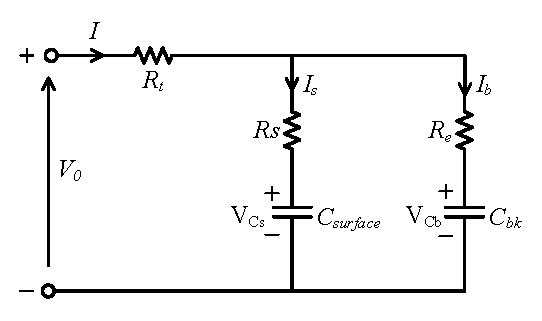
\includegraphics[width=0.7\linewidth]{rcmodel}
\end{figure}
\end{frame}

\begin{frame}{Columns and Blocks}

\begin{columns}

\column{0.4\textwidth}
    \begin{figure}[ht]
    \centering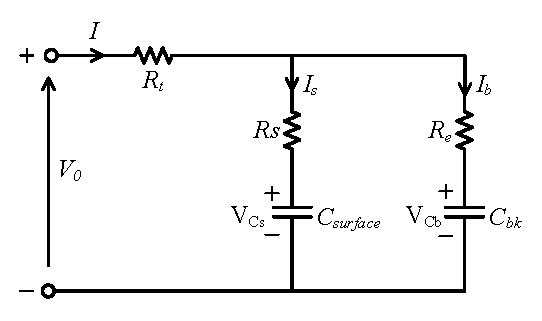
\includegraphics[scale=0.6]{rcmodel} 
    \caption{RC Model}
    \end{figure}

\column{0.5\textwidth} 
\begin{block}<1->{Observation 1}
Simmons Hall is composed of metal and concrete. 
\end{block}
\begin{block}<2->{Observation 2}
Simmons Dormitory is composed of brick.
\end{block}
      
\begin{block}<3->{Conclusion}
Simmons Hall $\not=$ Simmons Dormitory. \end{block}
\end{columns}

\end{frame}

\begin{frame}{Drawing in Beamer}
Refer to the latest manual, available for download via: \\
\url{http://www.texample.net/media/pgf/builds/}\\

\centering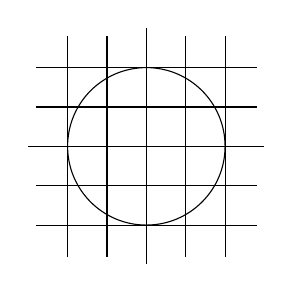
\begin{tikzpicture}
  \draw (-1.5,0) -- (1.5,0);
  \draw (0,-1.5) -- (0,1.5);
  \draw (0,0) circle (1cm);
  \draw[step=.5cm] (-1.4,-1.4) grid (1.4,1.4);
\end{tikzpicture}

\end{frame}

\begin{frame}{Video in Beamer}
Refer to the instructions from this website:\\

\url{https://tex.stackexchange.com/questions/345431/how-to-include-multimedia-files-in-beamer}

\end{frame}

%------------------------------------------------
\section{Theorem and Verbatim}
%------------------------------------------------

%Theorem
\begin{frame}{Theorem}
\begin{theorem}[Mass--energy equivalence]
$E = mc^2$
\end{theorem}
\end{frame}

\begin{frame}[<+->]{Theorem}
  \begin{theorem}
    $A = B$.
  \end{theorem}
  \begin{proof}
    \begin{itemize}
    \item Clearly, $A = C$.
    \item As shown earlier,  $C = B$.
    \item<-3>Thus $A = B$.
    \end{itemize}
  \end{proof}
\end{frame}

%------------------------------------------------

%Verbatim
\begin{frame}[fragile] % Need to use the fragile option when verbatim is used in the slide
{Verbatim}
\begin{example}[Theorem Slide Code]
\begin{verbatim}
\begin{frame}
\frametitle{Theorem}
\begin{theorem}[Mass--energy equivalence]
$E = mc^2$
\end{theorem}
\end{frame}\end{verbatim}
\end{example}


\end{frame}



%------------------------------------------------
\section{Citation and References}
%------------------------------------------------
% Citation
\begin{frame}[fragile] % Need to use the fragile option when verbatim is used in the slide
{Citation}
An example of the \verb|\cite| command to cite within the presentation:\\~

This statement requires citation \cite{p1}.
\end{frame}

% Reference
\begin{frame}
{References}
\footnotesize{
\begin{thebibliography}{99} % Beamer does not support BibTeX so references must be inserted manually as below
\bibitem[Smith, 2012]{p1} John Smith (2012)
\newblock Title of the publication
\newblock \emph{Journal Name} 12(3), 45 -- 678.
\end{thebibliography}
}
\end{frame}

%------------------------------------------------

\begin{frame}
\Huge{\centerline{The End}}
\end{frame}

%----------------------------------------------------------------------------------------

\end{document} 